\documentclass[tikz, border=0pt]{standalone}
\usepackage{tikz}
\usepackage{xcolor}
\usepackage{amsmath}

\definecolor{garnet}{HTML}{73000A}
\definecolor{atlantic}{HTML}{466A9F}
\definecolor{congaree}{HTML}{1F414D}
\definecolor{warmgrey}{HTML}{676156}
\definecolor{horseshoe}{HTML}{65780B}
\definecolor{bk70}{HTML}{5C5C5C}

\begin{document}
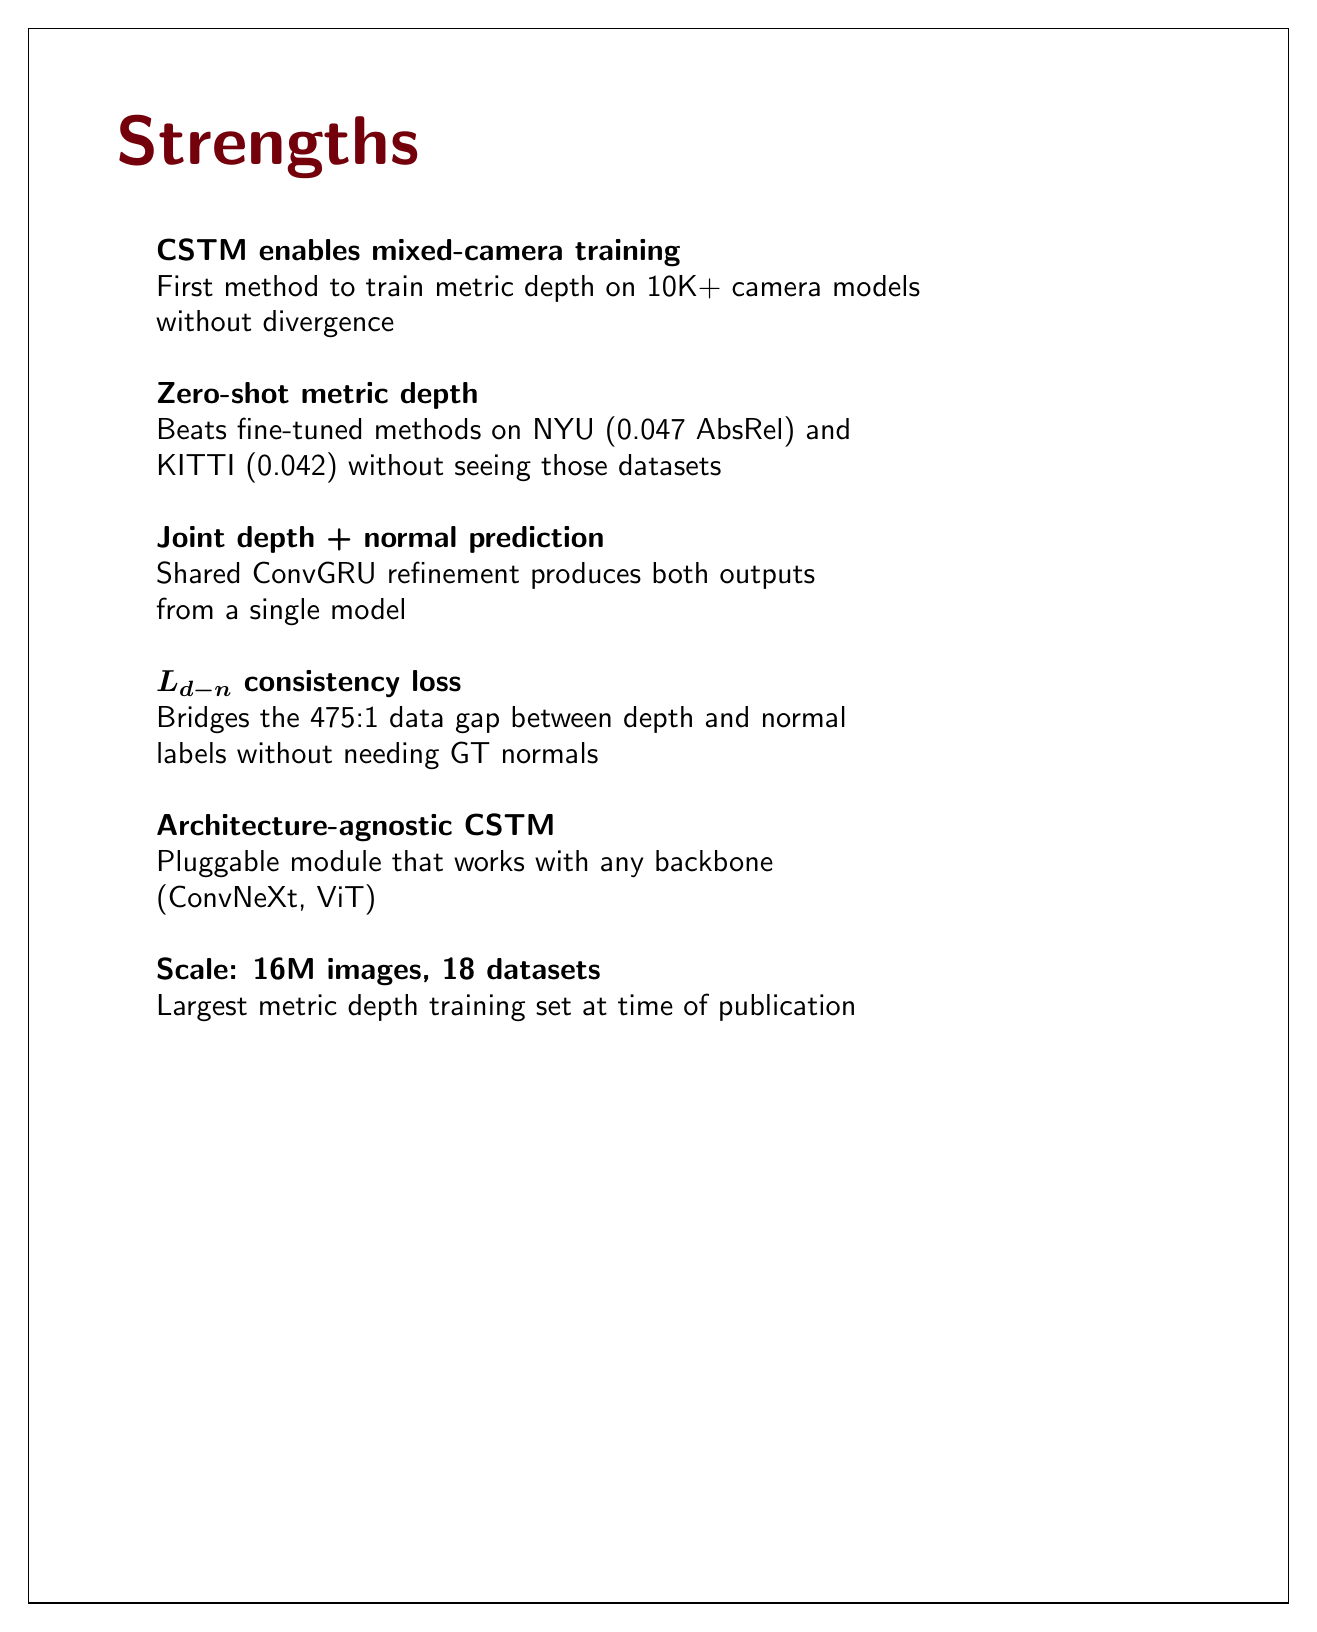
\begin{tikzpicture}[x=1cm, y=1cm]
  % Background
  \draw[fill=white] (0, 0) rectangle (16, 20);

  % Title
  \node[anchor=north west, font=\sffamily\bfseries\fontsize{40}{48}\selectfont, color=garnet]
    at (1, 19) {Strengths};

  % Content with bullet points
  \node[anchor=north west, font=\sffamily\fontsize{11}{13}\selectfont, color=black, align=left]
    at (1.5, 17.5) {
      \begin{tabular}{@{}l@{}}
        \textbf{CSTM enables mixed-camera training} \\
        First method to train metric depth on 10K+ camera models \\
        without divergence \\
        \\
        \textbf{Zero-shot metric depth} \\
        Beats fine-tuned methods on NYU (0.047 AbsRel) and \\
        KITTI (0.042) without seeing those datasets \\
        \\
        \textbf{Joint depth + normal prediction} \\
        Shared ConvGRU refinement produces both outputs \\
        from a single model \\
        \\
        \textbf{$\boldsymbol{L_{d-n}}$ consistency loss} \\
        Bridges the 475:1 data gap between depth and normal \\
        labels without needing GT normals \\
        \\
        \textbf{Architecture-agnostic CSTM} \\
        Pluggable module that works with any backbone \\
        (ConvNeXt, ViT) \\
        \\
        \textbf{Scale: 16M images, 18 datasets} \\
        Largest metric depth training set at time of publication
      \end{tabular}
    };

\end{tikzpicture}
\end{document}
